\scanpage{346}
\[
d,\ \lambda=\unsure{\overline T_\wedge|\overline T\wedge},\ \delta,\ \mu_i=T^{(i)}\cdot,
\quad\Theta(x)=\unsure{\deg(x)x}
\]
\[
1,T,\overline T
\]
\[
\deleted{\unsure{\Gamma\Phi\otimes\Lambda\Psi}}
\]
\[
\left\{\begin{aligned}
d\lambda+\lambda d&=0&&*\\
d\delta+\delta d&=\Theta\quad\text{\unsure{un opérateur}}\\
\delta\lambda+\lambda\delta&=\mu\\
d\mu_i-\deleted{\unsure{\mu_i d}}\mu_i d
 &=\deleted{\unsure{\lambda}}\mu_{i-1}\lambda\\
\lambda\mu_i+\mu_i\lambda&=0&&*\\
\delta\mu_i-\mu_i\delta&=0&&*
\end{aligned}\right.
\]
\[
A
\]
\[
d(T^{\unsure{(n)|n}}x)=
\underbrace{dT^{\unsure{(n)|n}}x}_{\unsure{\lambda T^{(n-1)}T_x}}
+T^{\unsure{n}}dx
\]
\[
d_f(x)\qquad d^\alpha\delta^\beta\lambda
\]
\[
\delta(Tx)=\deleted{\delta(T)x}+T\delta x
\]
\figure{\begin{tikzpicture}\draw (0,0)--(0,2);\end{tikzpicture}}
\[
\left\{\begin{aligned}
d\Theta-\Theta d&=0&&*\\
\delta\Theta-\Theta\delta&=0&&*\\
\Theta\lambda-\lambda\Theta&=\lambda\\
\Theta\mu_i-\mu_i\Theta&=i\mu_i
\end{aligned}\right.
\]
\figure{\begin{tikzpicture}\node[draw,ellipse,inner sep=8pt] {$\begin{gathered}
\Theta\mu_f-\mu_f\Theta=\mu_{\Theta f}\\
d\mu_f-\mu_f d=\mu_{f'}\lambda
\end{gathered}$};\end{tikzpicture}}
\[
\uline{d\lambda}\qquad\uline{\lambda\mu}\qquad\uline{\mu\delta}
\]
\figure{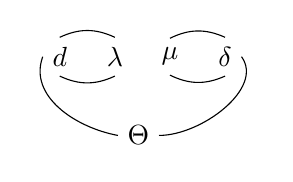
\begin{tikzpicture}
\node (d) at (0,0) {$d$};\node (l) at (.7,0) {$\lambda$};
\node (m) at (1.4,0) {$\mu$};\node (s) at (2.1,0) {$\delta$};
\node (o) at (1,-1) {$\Theta$};
\draw (d.north) to[bend left=25] (l.north);
\draw (m.north) to[bend left=25] (s.north);
\draw (d.south) to[bend right=25] (l.south);
\draw (m.south) to[bend right=25] (s.south);
\draw (d.west) .. controls (-.4,-.5) and (.2,-.9) .. (o.west);
\draw (s.east) .. controls (2.6,-.4) and (1.8,-1) .. (o.east);
\end{tikzpicture}}
\[
\frac{n(n-1)}2=\frac{5\cdot4}2=10
\qquad\frac{n(n+1)}2=\unsure{15|6}
\]
\[
d\ \delta\ \lambda\ \overset{i\ge1}{\mu_i}\ \Theta
\]
\[
\left\{\begin{aligned}
d^2=\delta^2=\lambda^2&=0\\
\mu_i\mu_j&=\unsure{C_{ij}}\mu_{i+j}
\end{aligned}\right.
\qquad\Theta^2\quad\text{\unsure{rien du tout}}
\]
\[
d,\delta,\lambda
\]
\figure{\begin{tikzpicture}
\draw[rounded corners=5pt] (-.6,1.1)--(7.4,1.4)--(7.4,-1.5)--(-.6,-1.7)--cycle;
\node (d) at (0,0) {$d$};\node (l) at (.8,0) {$\lambda$};
\node (m) at (1.7,0) {$\mu_f$};\node (s) at (2.6,0) {$\delta$};
\node (o) at (1.3,-1) {$\Theta$};
\draw (0,.25)--(0,.55)--(.7,.55)--(.7,.25);
\draw (.85,.25)--(.85,.55)--(1.65,.55)--(1.65,.25);
\draw (1.8,.25)--(1.8,.55)--(2.55,.55)--(2.55,.25);
\fill (.35,.8) circle (1pt);\fill (1.2,.8) circle (1pt);
\node at (2.7,1) {$\delta(T^{(i)})=0$};
\draw (d.south) .. controls (0,-.6) and (.6,-.8) .. (o.west);
\draw (s.south) .. controls (2.6,-.5) and (1.9,-1) .. (o.east);
\fill (-.1,-.9) circle (1pt);\fill (2.6,-.9) circle (1pt);
\node[anchor=west] at (3.2,-.2) {$\left\{\begin{aligned}
&\bullet\ d^2=\delta^2=\lambda^2=0\ \bullet\\
&\bullet\ \unsure{\mu_f\mu_g=\mu_{fg}},\quad\unsure{\mu_{f'}=f'\mu_1}\\
&\Theta^2=-
\end{aligned}\right.$};
\end{tikzpicture}}
\[
\unsure{\Theta|\Phi}(\lambda x)=(\deg x+i)\lambda x
\]
\[
\lambda(\unsure{\Theta|\Phi}x)=\deg x\ \lambda x
\]
\[
\unsure{\Theta|\Phi}\lambda-\lambda\unsure{\Theta|\Phi}=i\lambda x
\]
\[
\overset{A}{\sum}\lambda^\epsilon\cdot
\mu_{\unsure{f_{(\epsilon,}}}\ ;\ \delta^{\epsilon'}\Theta^n
\]
\figure{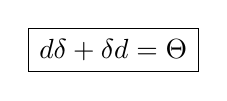
\begin{tikzpicture}\node[draw,inner sep=4pt] {$d\delta+\delta d=\Theta$};\end{tikzpicture}}
\[
\left\{\begin{aligned}
\delta\lambda+\lambda\delta&=\mu_T\\
d\mu_f-\mu_f d&=\mu_{f'}\lambda\quad\bullet\\
\Theta\lambda-\lambda\Theta&=\lambda\quad\bullet\\
\Theta\mu_f-\mu_f\Theta&=\mu_{\Theta f}\quad\bullet
\end{aligned}\right.
\]
\margin{$\delta(T)=1$}
\[
\sum_{\deleted{\unsure{\alpha,\beta,\sigma,n}}}
\mu_{f_{\unsure{\alpha\beta\sigma n}}}
\underbrace{\lambda^\alpha d^\beta\delta^\sigma\Theta^n}_{
\substack{\lambda^\epsilon d^{\epsilon'}\delta^{\epsilon''}\Theta^n\\
\unsure{\epsilon,\epsilon',\epsilon''}}}
\]
\margin{$\alpha,\beta,\sigma\in\unsure{\mathbb F_2}$\quad $n\in\mathbf N$}
\[
\deleted{\unsure{\mu_f}}
\]
\[
f\lambda^\alpha d^\beta\delta^\sigma\Theta^n
g\lambda^{\alpha'}d^{\beta'}\delta^{\sigma'}\Theta^{n'}
\]
\[
\lambda^\alpha\underbrace{d^\beta g}_{g d^\beta+\beta g'\lambda}
\delta^\sigma\lambda^{\alpha'}d^{\beta'}\delta^{\sigma'}
\]
Cas $p$ quelconque, $q=1$
\diagram{\begin{tikzcd}[column sep=large,row sep=large]
0\arrow[r,dash]&\Gamma^p\Phi_*\arrow[r]
&\Gamma^{\unsure{p-1}}\Phi_*\otimes\Phi_*\arrow[r,dash]
&\Gamma^{\unsure{p-1}}\Phi_*\otimes\Psi_*\arrow[r]
\arrow[l,bend left=35,"?",swap]&0\\
&&&\Phi_\alpha\times\Psi_\alpha\arrow[ul]&
\end{tikzcd}}
\diagram{\begin{tikzcd}
\Gamma^{\unsure{*+1|*+*}}\Phi_*\otimes\Lambda^*\Psi_*\arrow[d]\\
\Gamma^{\unsure{*+1|*+*}}\Phi_*\otimes\Lambda^*\Phi_*
\end{tikzcd}}
\[
(\varphi,\psi)\longrightarrow s(\varphi\otimes\psi)\varphi^{(p-1)}
\]
\[
\varphi_1^{(p_1)}-\varphi_r^{(p_r)}\qquad\sum p_i=p
\]
\diagram{\begin{tikzcd}[row sep=large]
\phantom{\varphi_1^{(p_1)}}\arrow[d]\\
\phantom{f(\varphi)}
\end{tikzcd}}
\[
\deleted{\sum\lambda_i\varphi_i}
\]
\[
\begin{aligned}
f\Bigl(\sum_i^r\lambda_i\varphi_i\Bigr)
&=s\Bigl(\sum\lambda_i\varphi_i\otimes\psi\Bigr)
\Bigl(\sum\lambda_i\varphi_i\Bigr)^{(p-1)}\\
&=\sum_{1\le i\le r}\lambda_i s(\varphi_i\otimes\psi)
\sum_{\substack{(p_1-p_r)\in\mathbf N^r\\\sum p_i=p-1}}
\lambda_1^{p_1}-\lambda_r^{p_r}\varphi_1^{(p_1)}-\varphi_r^{(p_r)}\\
&=\sum_{\substack{1\le i\le r\\(p_1-p_r)}}
\unsure{\lambda_i}\lambda_1^{p_1}\unsure{\lambda_i^{p_i}}\lambda_r^{p_r}
s(\varphi_i\otimes\psi)\varphi_1^{(p_1)}-\varphi_r^{(p_r)}
\end{aligned}
\]
\[
\varphi_1^{(q_1)}-\varphi_r^{(q_r)}\longmapsto
\sum_{\substack{\deleted{\unsure{1\le i\le r}}\\1\le\alpha\le r\\q_\alpha\ge1}}
s(\varphi_\alpha\otimes\psi)\varphi_1^{(q_1)}-
\varphi_\alpha^{(q_\alpha-1)}-\varphi_r^{(q_r)}
\]
\[
q_1\unsure{-|+\cdots+}q_r=p
\]
\diagram{\begin{tikzcd}[row sep=large]
\Gamma^2\Phi_*\otimes\Psi_*\arrow[d,bend left=35,"?"]\\
\Gamma^2\Phi_*\otimes\Phi_*\arrow[u]\\
\Gamma^2\Phi_*\arrow[u]\\
0\arrow[u]
\end{tikzcd}}
\diagram{\begin{tikzcd}[row sep=large]
\phantom{\Gamma^q(\Phi)}\\
\Gamma^q(\Phi)\otimes\unsure{\Phi|\Psi}\arrow[u]\arrow[d]\\
\Gamma^q(\Phi)\otimes\Psi'
\end{tikzcd}}
\figure{\begin{tikzpicture}\draw (0,0)--(2,2.8);\draw (0,-1.8)--(0,0);\end{tikzpicture}}
\[
\sum_{\unsure{\alpha\in\operatorname{Supp}q}}
\underbrace{(\varphi_\alpha\otimes\psi)
\varphi_1^{(q_1)}-\varphi_\alpha^{(q_\alpha-1)}-\varphi_r^{(q_r)}}_{
\displaystyle\sum q_\alpha\psi\varphi_1^{(q_1)}-\varphi_\alpha^{(q_\alpha)}-\varphi_r^{(q_r)}}
\]
\[
\Gamma^p\Phi_*,\quad\Lambda^q\Psi_*,\quad\Lambda^r\Phi_*,
\]
\figure{\begin{tikzpicture}\node[draw,ellipse] {$\Gamma^s\Psi_*\ ?$};\end{tikzpicture}}
\[
\unsure{\gamma_p|\gamma_\rho}(\psi\varphi_1^{(q_1)}-\varphi_n^{(q_n)})
\]
\[
\Phi_*,\Psi_*
\]
\[
\left\{\begin{aligned}
\Gamma^p\Phi_*\otimes\Lambda^q\Psi_*&=\mathrm{DR}_*^{p,q}\\
\Lambda^r\Phi_*&=C_*^{r,0}
\end{aligned}\right.
\]
\mspage{347}
